\RequirePackage[dvipsnames]{xcolor}
\documentclass[shortabstract, inz]{iithesis}

\usepackage[utf8]{inputenc}

%%%%% DANE DO STRONY TYTUŁOWEJ
\polishtitle    {Poker Master Tool --- Sieciowy kalkulator \fmlinebreak układów dla Texas Holdem}
\englishtitle   {Poker Master Tool --- Web hand calculator for Poker Texas Holdem}
\polishabstract {
Celem pracy jest stworzenie kalkulatora układów dla gry Poker Texas Holdem. Wyzwaniem jest przygotowanie szybko działającego rozwiązania w środowisku webowym. Aplikacja ma także na celu zaprojektowanie intuicyjnego interfejsu użytkownika, które zachęci graczy do poznawania teorii pokera.
Praca zawiera wprowadzenie do gry poker Texas Holdem, wyjaśnia działanie ewaluatorów oraz kalkulatorów szans, opisuje implementację i architekturę rozwiązania oraz zawiera instrukcję użytkownika.
}
\englishabstract{
The purpose of the thesis is creation poker hand calculator for Texas Holdem. The challenge is preparing a fast solution in a web environment. Another goal is to encourage players to expand their knowledge and therefore the application should contain an intuitive user interface. The paper includes an introduction to the card game Poker Texas Holdem, explains the mechanism of poker evaluators and calculators, describes the implementation and architecture of the software with a user manual.
}
\author         {Bartosz Putek}
\advisor        {dr hab. Artur Jeż}
\date          {23 czerwca 2022}                     % Data zlozenia pracy
% Dane do oswiadczenia o autorskim wykonaniu
\transcriptnum {308946}                     % Numer indeksu
\advisorgen    {dr hab. Artura Jeża} % Nazwisko promotora w dopelniaczu
%%%%%

%%%%% WLASNE DODATKOWE PAKIETY
%
\usepackage{graphicx, fdsymbol}
\usepackage[dvipsnames]{xcolor}
\usepackage{tikz}
\usepackage{fancyvrb}
\usepackage{listings}
\usepackage{hyperref}
\usepackage{booktabs}
\usetikzlibrary{shapes.geometric, arrows}

%
%%%%% WŁASNE DEFINICJE I POLECENIA
%

\newcommand{\clubs}{\textcolor{OliveGreen}{\clubsuit}}
\newcommand{\spades}{\spadesuit}
\newcommand{\hearts}{\textcolor{red}{\varheartsuit}}
\newcommand{\diamonds}{\textcolor{blue}{\vardiamondsuit}}

\tikzstyle{process} = [rectangle, minimum width=3cm, minimum height=1cm, text centered, text width=3.3cm, draw=black, fill=orange!30]
\tikzstyle{arrow} = [thick,->,>=stealth]

\lstset{frame=single, numbers=left}

%%%%%

\begin{document}

\chapter{Wstęp}
\label{chapter:1}

\section{Zawartość pracy}

\hyperref[chapter:1]{Pierwszy rozdział} zawiera wprowadzenie wyjaśniające jaki problem rozwiązuje aplikacja \emph{Poker Master Tool}.
\hyperref[chapter:2]{Drugi rozdział} objaśnia zasady gry Poker Texas Hold’em, wyjaśnia działanie kalkulatorów szans oraz zawiera porównanie z innymi istniejącymi rozwiązaniami.
\hyperref[chapter:3]{Trzeci rozdział} opisuje algorytm wykorzystany w silniku aplikacji.
W \hyperref[chapter:4]{czwartym rozdziale} omówiono implementację rozwiązania.
\hyperref[chapter:5]{Piąty rozdział}  to instrukcja użytkownika z demonstracyjnymi przypadkami użycia.
W \hyperref[chapter:6]{szóstym rozdziale} zostało zawarte podsumowanie.

\section{Opis problemu i cel powstania aplikacji}

Poker \cite{wiki-poker} to jedna z najpopularniejszych gier karcianych na świecie. Codziennie grają w niego miliony graczy online oraz na żywo. Kluczowymi umiejętnościami jest dobór odpowiedniej strategii, znajomość elementów rachunku prawdopodobieństwa oraz aspekty psychologiczne. Aby udoskonalać swoją strategię, profesjonalni pokerzyści korzystają z szerokiej gamy narzędzi. Jedną z kategorii takich aplikacji są kalkulatory szans (ang. equity calculator), które służą do obliczenia szans wygranej dla poszczególnych graczy przy zadanych kartach graczy oraz kartach wspólnych. Dzięki temu gracze mogą ocenić siłę swojej ręki co ułatwia im podejmowanie decyzji.

Niestety, większość kalkulatorów obecnych na rynku jest nieprzyjazna dla amatorów pokera --- zawierają zbyt dużo skomplikowanych opcji, a ich interfejs jest nieczytelny, przez co próg wejścia jest wysoki, jeżeli gracz zechciałby zacząć ich używać. Większość kalkulatorów jest dostępna tylko jako aplikacja desktopowa, a inne w formie aplikacji webowej (sieciowej) są nieprzystosowane do szerokości ekranów urządzeń mobilnych. 

\emph{Poker Master Tool} stara się rozwiązać ten problem --- jest to w pełni responsywna aplikacja webowa, z interfejsem dostosowanym do współczesnych standardów, oferująca kalkulację szans na wygraną i szans uzyskania poszczególnych układów. Dzięki prostocie obsługi kalkulatora, mniej doświadczeni gracze mają szansę z zaznajomieniem się z teorią pokera. 

Aplikacja dostępna jest pod adresem \href{https://pokermastertool.bartoszputek.pl/}{https://pokermastertool.bartoszputek.pl/}, a kod źródłowy na repozytorium \href{https://github.com/bartoszputek/poker-master-tool/}{https://github.com/bartoszputek/poker-master-tool/}.


\chapter{Poker oraz kalkulatory szans}
\label{chapter:2}

\section{Zasady gry Poker Texas Hold’em}

Poker Texas Hold’em \cite{wiki-texas-holdem} to najpopularniejsza odmiana pokera. W standardowej rozgrywce uczestniczy od 2 graczy do 9 graczy oraz używa się pełnej talii 52 kart. Celem gry jest wygranie żetonów od innych graczy poprzez skompletowanie silniejszego układu bądź wymuszenie spasowania kart od pozostałych graczy. Każdy z graczy dysponuje dwiema kartami oraz kartami wspólnymi ujawnianymi w kolejnych rundach licytacji. Gracze w każdej turze licytacji mają do dyspozycji następujące możliwości:

\begin{itemize}
    \item Spasowanie kart (fold)
    \item Sprawdzenie (call)
    \item Podbicie stawki (raise)
    \item Czekanie (check)
\end{itemize}

Gracz może czekać tylko, gdy w obecnej turze licytacji nikt wcześniej nie podbił stawki (raise). Pojedyncze rozdanie składa się z co najwyżej 4 tur licytacji, po których dochodzi do ujawnienia kolejno: trzech kart wspólnych (flop), jednej karty wspólnej (turn) i ostatniej kart wspólnej (river). Po ostatniej turze licytacji odbywa się określenie siły rąk wszystkich graczy pozostałych w rozdaniu.

\begin{figure}[ht]
    \fbox{ \scalebox{0.74}{\includegraphics{images/example-hand.png}}}
    \caption{Przykładowy stan gry w trakcie ostatniej tury licytacji (river)}
    \label{fig:example-hand}
\end{figure}

Ewaluacja ręki polega na określeniu układu z poniższej listy rankingowej. Każdy z graczy do określenia swojego układu wybiera pięć kart spośród dwóch kart własnych i pięciu wspólnych.

Układy kart od najsłabszego:
\begin{description}
  \item[Wysoka karta] (High Card): Następuje w przypadku gdy układ nie kwalifikuje się pod żaden z poniższych. Gracz wybiera 5 najwyższych dostępnych dla siebie kart. Jeżeli obydwoje z graczy mają wysoką kartę należy porównać kolejno najwyższe karty. W przypadku identycznego układu następuje remis. Podobną zasadę (kicker) stosuje się w przypadku remisów w innych układach, które należy uzupełnić do 5-kartowego układu. (np. $A\clubs, T\diamonds, 7\spades, 5\hearts, 2\hearts$)
  \item[Para] (One pair): dwie karty o tej samej wartości; jeżeli gracze mają tą samą parę, decyduje kicker. (np. $A\clubs, A\diamonds, J\diamonds, 9\spades, 2\spades$)
  \item[Dwie pary] (Two pairs): Wygrywa gracz z wyższą parą; jeżeli najwyższa para jest identyczna, to wygrywa gracz z drugą najwyższą parą. Gdy druga para jest identyczna --- decyduje kicker. (np. $K\clubs, K\diamonds, T\spades, T\hearts, 4\hearts$)
  \item[Trójka] (Three of a Kind): Wygrywa gracz z trójką o wyższej randze; jeżeli ranga jest ta sama, to decyduje kicker. (np. $K\clubs, K\diamonds, K\spades, 7\hearts, 4\hearts$)
  \item[Strit] (Straight): pięć kolejnych kart; jeśli dwóch graczy ma strita to wygrywa ten, który ma wyższą kartę. W stricie as może być zarówno najwyższą jak i najniższą kartą --- jedynką. (np. $A\spades, K\diamonds, Q\clubs, J\spades, T\hearts$)
   \item[Kolor] (Flush): pięć kart w tym samym kolorze; jeśli dwóch graczy ma kolor (uzyskanie dwóch różnych kolorów jest niemożliwe) wygrywa ten, którego kolor ma najwyższą kartę. (np. $K\spades, T\spades, J\spades, 8\spades, 7\spades$)
   \item[Full] (Full house): układ składający się z trójki oraz pary; jeśli dwóch graczy ma fulla, to wygrywa ten, który ma wyższą trójkę; jeśli obydwaj mają tę samą trójkę, wygrywa ten, który ma wyższą parę; jeśli i para jest taka sama, to następuje remis. (np. $K\clubs, K\diamonds, K\spades, 4\hearts, 4\diamonds$)
  \item[Kareta] (Quads): cztery karty tej samej rangi; jeżeli obydwoje z graczy mają karetę, wygrywa ten składający się z wyższej rangi. (np. $K\clubs$, $K\diamonds$, $K\spades$, $K\hearts, 2\diamonds$)
  \item[Poker] (Straight flush): pięć kolejnych kart w tym samym kolorze; jeżeli obydwoje z graczy mają pokera, wygrywa ten z ostatnią wyższą kartą. (np. $Q\hearts, J\hearts,$ $T\hearts, 9\hearts, 8\hearts$)
\end{description}
 
\newpage{}

W scenariuszu przedstawionym na rysunku \ref{fig:example-hand} gracze dysponują następującymi układami:
\begin{itemize}
    \item Player 1: Para dziesiątek --- $T\clubs, T\hearts, K\spades, Q\spades, 9\diamonds $
    \item Player 2: Para dziesiątek --- $T\clubs, T\hearts, A\diamonds, 9\diamonds, 6\spades $
    \item Player 3: Dwie pary --- $T\clubs, T\hearts, 8\clubs, 8\spades, 9\diamonds $
\end{itemize}

Zatem gracz trzeci dysponuje najlepszym układem, drugi po nim jest gracz numer dwa, a najgorszym układem dysponuje gracz numer jeden (gracz numer dwa posiada wyższego kickera --- $A\diamonds > K\spades$).

\section{Działanie kalkulatora szans}

Zadaniem kalkulatorów szans (ang. equity calculator) jest obliczenie szansy na wygraną każdego z graczy przy wybranych przez użytkownika kartach graczy oraz kartach wspólnych --- taką sytuację dalej nazwiemy \emph{scenariuszem}. Zatem zakładamy, że każdy gracz uczestniczący w rozdaniu będzie podejmował tylko jedną akcję --- check. Wyniki z kalkulatora przydają się, do określenia rzeczywistej siły ręki przeciwko innym rękom np. przy zagraniu za wszystko (all-in) w sytuacji $Q\spades, K\spades$ vs $A\spades, A\clubs$ z kartami wspólnymi $5\diamonds, 6\hearts, Q\clubs$ gracz pierwszy ma tylko 18\% szans na wygraną.

\begin{figure}[ht]
    \fbox{ \scalebox{0.94}{\includegraphics{images/example-hand-2.png}}}
    \caption{Wizualizacja powyższego scenariusza}
    \label{fig:example-hand-2}    
\end{figure}

Kalkulatory szans bazują na podobnej zasadzie. Należy określić, jakie karty są dostępne w talii, a następnie rozpatrzyć wszystkie możliwe kombinacje i w każdej z nich określić zwycięzcę. W scenariuszu przedstawionym na rysunku \ref{fig:example-hand-2} w talii pozostało 45 kart (52 minus po dwie karty każdego z graczy i trzy na stole). Musimy wybrać dwie z nich zatem liczba kombinacja bez powtórzeń to $\binom{45}{2}= 990$. Dla tak prostego scenariusza problem jest łatwy, natomiast w pesymistycznym i najczęstszym przypadku użycia, gdy kart w talii jest najwięcej oraz na stole nie ma żadnych kart, liczba kombinacji drastycznie rośnie, nawet do $\binom{48}{5}= 1712304$ kombinacji.

Naiwne podejście do tego problemu jest naturalne. W każdej kombinacji można posortować karty każdego z graczy, przyjrzeć się pojedynczo każdej z kart i zebrać w ten sposób potrzebne dane (np. zliczać kolory, pary) do ustalenia układu. Ten sposób ma jedną poważną wadę - jest zdecydowanie zbyt wolny do zastosowania w scenariuszach z wieloma kombinacjami. 

Wszystkie szybkie kalkulatory szans wykorzystują zapamiętane wcześniej wyniki przez naiwny algorytm lub korzystają z metody Monte Carlo \cite{monte-carlo} \cite{monte-carlo-presentation} do przybliżania wyników przy dostatecznie małym błędzie. Aplikacja  \emph{Poker Master Tool} oblicza wynik dokładnie, zatem będziemy się zajmować tylko tą metodą.

\section{Porównanie z innymi dostępnymi kalkulatorami}

\subsection{Poker Master Tool}

\href{https://pokermastertool.bartoszputek.pl/}{\emph{Poker Master Tool}} jest aplikacją internetową opartą o architekturę klient-serwer. Klient z poziomu przeglądarki w wygodny sposób wybiera interesujący go scenariusz, a następnie informacje są wysyłane do serwera, który dane przetwarza i zwraca wyświetlaną w widoku użytkownika odpowiedź. Z tego powodu do korzystania z aplikacji niezbędne jest połączenie internetowe. 

Użytkownik za pomocą myszy lub klawiatury jest w stanie wybrać karty dla każdego z graczy, karty wspólne oraz tak zwane karty martwe, wykluczone z pozostałej części talii. Informacje jakie dostajemy w zwrotnej odpowiedzi to:
\begin{itemize}
    \item Szanse na wygraną, przegraną oraz remis każdego z graczy
    \item Szanse na poszczególne układy każdego z graczy
    \item Liczbę kombinacji w danym scenariuszu
\end{itemize}

\begin{figure}[!htbp]
    \fbox{ \scalebox{0.22}{\includegraphics{images/poker-master-tool-view.png}}}
    \caption{Standardowy widok aplikacji Poker Master Tool}
    \label{fig:poker-master-tool-view}    
\end{figure}

\subsection{Power Equilab}

\href{http://power-equilab.com/}{\emph{Power Equilab}} jest płatnym oprogramowaniem przeznaczonym dla profesjonalistów w formie aplikacji desktopowej. Nie posiada wersji na telefony, za to w odróżnieniu od aplikacji webowej nie potrzebuje do działania połączenia z internetem. Jedną z jego funkcjonalności jest kalkulator szans. Kalkulator posiada wiele rozbudowanych opcji, które mogą być niejasne z perspektywy początkującego gracza, lecz bardzo przydatne dla graczy zaawansowanych. Interfejs aplikacji niestety nie pozwala komfortowo korzystać z klawiatury. 

\begin{figure}[!htbp]
    \scalebox{0.75}{\includegraphics{images/power-equilab-view.png}}
    \caption{Standardowy widok aplikacji Power Equilab}
    \label{fig:power-equilab-view}    
\end{figure}

\subsection{Card Player Poker Odds Calculator}

\href{https://www.cardplayer.com/poker-tools/odds-calculator/texas-holdem/}{\emph{Card Player Poker Odds Calculator}} jest webowym kalkulatorem szans. Jego główną zaletą jest prostota oraz brak konieczności instalacji oprogramowania na własnym komputerze. Niestety, mimo architektury webowej trudno z niego korzystać na urządzeniach mobilnych. Nie posiada żadnych zaawansowanych funkcji oraz wynik zawiera tylko kalkulację szansy na zwycięstwo dla każdego z graczy. Interfejs nie wspiera obsługi klawiatury, a aplikacja wymaga stałego połączenia internetowego, podobnie jak w przypadku \emph{Poker Master Tool}.

\begin{figure}[!htbp]
    \scalebox{0.68}{\includegraphics{images/card-player-view.png}}
    \caption{Standardowy widok aplikacji Card Player Poker Odds Calculator}
    \label{fig:card-player-view}    
\end{figure}

\begin{table}[h]
    \centering
    \begin{tabular}{lllll}
        {} & Poker Master Tool & Power Equilab & Card Player Calc.\\
        \midrule
        Typ aplikacji & Webowa  & Desktopowa & Webowa \\
        Połączenie internetowe & Tak & Nie & Tak \\
        Obsługa klawiatury & Tak & Nie & Nie \\
        Liczba funkcji & Średnia & Duża & Niska \\
        Urządzenia mobilne & Tak & Nie & Nie \\
        Przeznaczenie & Początkujący & Profesjonaliści & Początkujący \\
        Model & Darmowy & Płatny & Darmowy \\
        \bottomrule
    \end{tabular}
    \caption{Podsumowanie prezentowanych kalkulatorów}
\end{table}

\chapter{Ewaluacja układów}
\label{chapter:3}

\section{Wprowadzenie}

Podstawą działania kalkulatorów szans jest algorytm odpowiedzialny za określanie siły ręki. W przypadku odmiany Poker Texas Hold’em należy określić ją na podstawie 7 kart - 2 gracza oraz 5 wspólnych. Program, który realizuje powyższe zadanie nazwiemy ewaluatorem. Szybkość ewaluacji jest najistotniejsza z punktu widzenia naszej aplikacji, ponieważ to właśnie ten proces zajmuje zdecydowaną większość czasu odpowiedzi serwera.

\section{Ewaluator Cactus Kev's}

Kevin Suffecool, autor ewaluatora \emph{Cactus Kev's} \cite{cactus-kev-evaluator} \cite{cactus-kev-equivalence-classes} zauważył, że 5-kartowe kombinacje, których jest $\binom{52}{5}= 2598960$ można pogrupować w według ich siły. Na przykład układ $A\clubs, K\clubs, Q\clubs, J\clubs, T\clubs$ jest identyczny pod względem siły z $A\hearts, K\hearts, $ $Q\hearts, J\hearts, T\hearts$, gdyż każdy z układów to najwyższy możliwy do uzyskania poker. Grupując w taki sposób wszystkie możliwe kombinacje uzyskujemy tylko 7462 porównywalnych wartości. Grupy te nazwiemy \emph{klasami równoważności}.

\begin{table}[htbp]
    \centering
    \begin{tabular}{lll}
        Układ & Unikalne & Zredukowane \\
        \midrule
        Poker          & 40                         & 10  \\
        Kareta         & 624                        & 156   \\
        Full           & 3744                       & 156  \\
        Kolor          & 5108                       & 1277 \\
        Strit          & 10200                      & 10 \\
        Trójka         & 54912                      & 858  \\
        Dwie pary      & 123552                     & 858  \\
        Para           & 1098240                    & 2860 \\
        Wysoka karta   & 1302540                    & 1277 \\
        \bottomrule
        Razem          & 2598960                    & 7462 \\
        \bottomrule
    \end{tabular}
    \caption{\label{tab:catus-kev-reduction}Redukcja 5-kartowych kombinacji według ich siły}
\end{table}


Ewaluator \emph{Cactus Kev's} przyjmując 5 kart zwraca liczbę od 1 do 7462, reprezentującą układ, gdzie 1 oznacza najsilniejszy układ, a 7462 najsłabszy.

Pojedyncza karta reprezentowana jest jako 32 bitowa liczba:

\scalebox{0.6}{
    \begin{tabular}{|l|l|l|l|l|l|l|l|l|l|l|l|l|l|l|l|l|l|l|l|l|l|l|l|l|l|l|l|}
    \hline
    - & - & - & B & B & B & B & B & B & B & B & B & C & D & H & S & R & R & R & R & X & X & P & P & P & P & P & P \\ \hline
    \end{tabular}
}

gdzie:

\begin{itemize}
    \item Pierwsze 6 bitów P reprezentują rangę karty jako liczba pierwsza (dwójka - 2, trójka - 3, czwórka - 5, ... , as - 41)
    \item Cztery bity R reprezentują rangę karty jako kolejna liczba naturalna (dwójka - 1, trójka - 2, czwórka - 3, ... , as - 12), nie są one wykorzystywane przez ewaluator w żaden sposób \label{chapter:3-r-bits}
    \item Jeden z zapalonych bitów CDHS oznacza kolor karty (C - trefl, D - karo, H - kier, S - pik)
    \item Dwanaście bitów B reprezentuję rangę karty jako kolejny zapalony bit (pierwszy zapalony bit to dwójka, drugi to trójka itd.)
\end{itemize}

Karty otrzymane na wejściu w powyższym formacie oznaczmy kolejno jako $C1$, $C2$, $C3$, $C4$, $C5$. W pierwszej kolejności ewaluator sprawdza, czy wszystkie karty są tego samego koloru korzystając z poniższej formuły:

\begin{verbatim}
isSuited = C1 AND C2 AND C3 AND C4 AND C5 AND 0xF000
\end{verbatim}

Jeżeli wartość \verb+isSuited+ nie jest równa zero, to wszystkie karty są tego samego koloru. W przypadku gdy układ jest kolorem lub pokerem obliczenie wartości polega na zajrzenie do tablicy \verb+flushes+, w której indeksem jest wyrażenie \verb+index+. Na przykład wartość przechowywana w tablicy \verb+flushes[0x1F00]+ jest równa 1, gdyż 1 jest \emph{klasą równoważności} odpowiadającą asowemu pokerowi.

\begin{verbatim}
index = (C1 OR C2 OR C3 OR C4 OR C5) >> 16
\end{verbatim}

Zauważmy, że najmniejsza możliwa wartość wyrażenia \verb+index+ to \verb+0x001F+ (31), a największa \verb+0x1F00+ (7936). Tablica \verb+flushes+ ma zatem długość 7936 i została wypełniona obliczonymi wcześniej \emph{klasami równoważności} za pomocą naiwnego algorytmu. Większość komórek w naszej tablicy to puste wartości, gdyż możliwych kolorów i pokerów jest $\binom{13}{5}= 1287$. W technice tablicowania \cite{lookup-tables} zyskujemy szybkość działania, w zamian za niewykorzystaną pamięć. 

W przypadku, gdy wszystkie karty nie są tego samego koloru, możemy użyć tej samej techniki do sprawdzenia układów zawierające same unikalne karty --- Strit oraz Wysoka karta. Została skonstruowana tablica \verb+unique5+ zawierająca porównywalne wartości dla Strita oraz Wysokiej karty. Jej długość oraz indeksy pod którymi znajdują się niezerowe wartości są identyczne z tablicą \verb+flushes+, ponieważ układy poker --- strit, kolor --- wysoka karta różnią się tylko obecnością koloru. Indeksem w tej tablicy jest wartość wyrażenia \verb+index+. Oznacza to, że pod indeksem \verb+flushes[0x1F00]+ znajduje się wartość 1600, która oznacza asowego strita.

Pozostają nam układy, w których występuje co najmniej jedno powtórzenie karty o tej samej randze. Do obliczenia takich układów posłużą nam bity P, reprezentujące poszczególne rangi jako liczby pierwsze.
Aby uniknąć kosztownego sortowania kart, ewaluator korzysta z Podstawowego twierdzenia arytmetyki \cite{theorem-of-arithmetic} oraz przemienności mnożenia.

\begin{verbatim}
product = (C1 AND 0xFF) * (C2 AND 0xFF) * (C3 AND 0xFF) * 
        (C4 AND 0xFF) * (C5 AND 0xFF)
\end{verbatim}

Największa wartość wyrażenia \verb+product+ to $41^4 \cdot 37=104553157$, zatem skonstruowanie tak dużej tablicy będzie wymagało za dużo pamięci. Autor rozwiązania obliczył wszystkie iloczyny liczb pierwszych dla pozostałych 4888 układów (7462-2574), posortował je oraz zapisał w tablicy \verb+products+. Następnie jest wyszukiwana binarnie \cite{binary-search} wartość \verb+product+ w tablicy, a otrzymany w ten sposób indeks posłuży nam jako indeks w tablicy \verb+value+, w której znajdują się wcześniej obliczone przez naiwny algorytm \emph{klasy równoważności}.

\section{Poprawa wydajności Paula Senzee'a}

Paul Senzee \cite{paul-senzee-improvements} zauważył, że ostatni krok algorytmu jest najbardziej czasochłonny oraz większość rąk wymaga jego wykonania. Zastąpił on zatem wyszukiwanie binarne korzystając z doskonałej minimalnej funkcji haszującej \cite{minimal-perfect-hash-function}. Skonstruował ją za pomocą programu do generowania tablic haszujących autorstwa Boba Jenkinsa \cite{bob-jenkins-hashing}. Dodatkowo, w sposób naiwny dodał możliwość ewaluacji 6 i 7 kartowych układów wywołując obliczenia dla każdej możliwej kombinacji i zwrócenie maksymalnej wartości.

\section{Ewaluator TwoPlusTwo}

W 2006 roku na jednym z najpopularniejszych forów pokerowych \emph{TwoPlusTwo} \cite{twoplustwo-thread} \cite{poker-hand-evaluator-roundup} została rozpoczęta praca nad \emph{ewaluatorem} przeznaczonym do sekwencyjnego obliczania siły układów. Ideą jest wykorzystanie wcześniej obliczonych częściowych wyników, aby jeszcze bardziej przyspieszyć proces ewaluacji dla dużej liczby kombinacji. 

Ewaluator \emph{TwoPlusTwo} skupia się na konstrukcji automatu skończonego \cite{finite-state-machine}, w którym kolejne przejścia wyznaczane są na podstawie kolejnych kart. Od piątego wierzchołka możliwe jest zwrócenie typu układu razem z jego miejscem w rankingu względem tych samych układów. Na przykład dla asowego strita zwrócona zostanie kategoria 5, gdyż strit jest 5 układem licząc od najsłabszego oraz ranga 10, gdyż jest najwyższym stritem, a rozróżnialnych stritów jest 10. Podczas konstruowania grafu wykorzystywany jest ewaluator Cactus Kev razem z poprawkami Paul'a Senzee do obliczania siły układów . 


\begin{figure}[h]
\centering
\fbox{ 
    \begin{tikzpicture}[node distance=2cm]
    
    \node (pro1) [process] {$3\diamonds 4\spades 5\hearts A\spades$};
    \coordinate[below of=pro1] (c1);
    \coordinate[left of=c1] (c2);
    \coordinate[right of=c1] (c3);
    \node (pro2) [process, left of=c2] {$2\diamonds 3\diamonds 4\spades 5\hearts A\spades$};
    \node (pro2a) [process, below of=pro2] {Kategoria: 5 Ranga: 1 \\ Piątkowy strit};
    \node (pro3) [process, right of=c2] {$3\spades 3\diamonds 4\spades 5\hearts A\spades$};
    \node (pro3a) [process, below of=pro3] {Kategoria: 2 Ranga: 388 \\ Para trójek};
    \node (pro4) [process, right of=c3] {$3\diamonds 4\spades 4\hearts 5\hearts A\spades$};
    \node (pro4) [process, right of=c3] {$3\diamonds 4\spades 4\hearts 5\hearts A\spades$};
    \node (pro4a) [process, below of=pro4] {Kategoria: 2 Ranga: 608 \\ Para czwórek};
    
    \draw [arrow] (pro1) -- node[midway, above, sloped] {$2\diamonds$}(pro2);
    \draw [arrow] (pro1) -- node[anchor=west] {$3\spades$}(pro3);
    \draw [arrow] (pro1) -- node[midway, above, sloped] {$4\hearts$}(pro4);
    \draw [arrow] (pro2) -- (pro2a);
    \draw [arrow] (pro3) -- (pro3a);
    \draw [arrow] (pro4) -- (pro4a);
    \draw [arrow, <-] (pro1) -- node[above, anchor=west] {...} ++(0cm,2cm);
    
    \end{tikzpicture}
}
\caption{Przykładowa część grafu}
\label{fig:graph-1}
\end{figure}

Tworzenie grafu wykorzystuje dwie poniższe techniki, redukujące znacząco liczbę wierzchołków:

\begin{itemize}
    \item Te same karty ułożone w dowolnej kolejności wskazują na ten sam wierzchołek (rysunek \ref{fig:graph-2})
    
    \begin{figure}[h]
    \centering
    \fbox{ 
        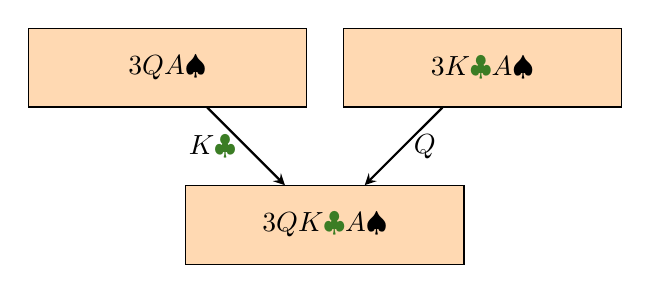
\begin{tikzpicture}[node distance=2cm]
        \coordinate[] (c1);
        \node (pro1) [process, right of=c1] {$3\diamonds K\clubs A\spades$};
        \node (pro2) [process, left of=c1] {$3\diamonds Q\diamonds A\spades$};
        \node (pro3) [process, below of=c1] {$3\diamonds Q\diamonds K\clubs A\spades$};
        
        \draw [arrow] (pro2) -- node[anchor=east] {$K\clubs$}(pro3);
        \draw [arrow] (pro1) -- node[anchor=west] {$Q\diamonds$}(pro3);
       
        \end{tikzpicture}
    }
    \caption{Te same karty w różnej kolejności wskazują na ten sam wierzchołek}
    \label{fig:graph-2}   
    \end{figure}
    
    \item Aby kolor był znaczący $n-2$ kart musi być tego samego koloru, gdzie $n$ to długość układu. Gdy kolor jest nieznaczący następuje redukcja wierzchołków, ignorując kolor we wszystkich kartach.
\end{itemize}

\begin{figure}[h]
\centering
\fbox{ 
    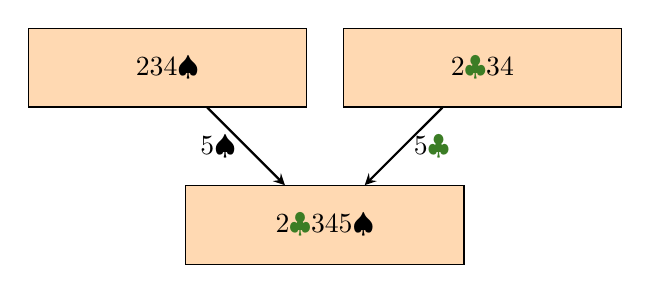
\begin{tikzpicture}[node distance=2cm]
    \coordinate[] (c1);
    \node (pro1) [process, right of=c1] {$2\clubs 3\diamonds 4\hearts$};
    \node (pro2) [process, left of=c1] {$2\diamonds 3\hearts 4\spades$};
    \node (pro3) [process, below of=c1] {$2\clubs 3\diamonds 4\hearts 5\spades$};
    
    \draw [arrow] (pro2) -- node[anchor=east] {$5\spades$}(pro3);
    \draw [arrow] (pro1) -- node[anchor=west] {$5\clubs$}(pro3);
    
    \end{tikzpicture}
}
\caption{Redukcja wierzchołków po wykryciu nieznaczącego koloru. Dla 4 kartowego układu, aby kolor był znaczący przynajmniej dwie karty powinny mieć ten sam kolor.}
\label{fig:graph-3}
\end{figure}

Aplikując powyższe zasady, graf zawiera 32487834 wierzchołków, przez co jego rozmiar na dysku to około 123 MB, w zamian uzyskując bardzo szybką ewaluację układów.
Korzystając z ewaluatora \emph{TwoPlusTwo} wystarczy tylko 7 odczytów z naszego grafu, aby uzyskać siłę ręki dla 7 kartowego układu. 

W poniższych pseudokodach wykorzystane są następujące oznaczenia zmiennych:

\begin{description}
  \item[Cards] jest zmienną zawierającą karty, dla których chcemy uzyskać siłę układu.
  \item[HR] to automat skończony reprezentowany jako tablica.
  \item[Pointer] oznacza zmienną, która wskazuje na aktualny element w grafie.
  \item[Value] jest obliczoną siłą naszego układu.
\end{description}

\begin{Verbatim}[numbers=left,xleftmargin=5mm, frame=single]
int LookupHand(int* cards)
{
    int pointer = HR[53 + *cards++];
    pointer = HR[pointer + *cards++];
    pointer = HR[pointer + *cards++];
    pointer = HR[pointer + *cards++];
    pointer = HR[pointer + *cards++];
    pointer = HR[pointer + *cards++];
    
    int value = HR[pointer + *playerCards++];
    
    return value;
}
\end{Verbatim}

Dodatkowo sekwencyjne przeszukiwanie rąk jest bardzo szybkie wykorzystując wcześniej otrzymane wskaźniki. Na przykład posiadając karty $3\hearts, T\spades, Q\clubs, A\diamonds$ chcemy obliczyć wszystkie możliwe 5-kartowe uzupełnienia . Obliczamy zatem wskaźnik do wcześniej wymienionego układu, a następnie przechodzimy po wszystkich pozostałych kartach w talii, wykorzystując ten wskaźnik:

\begin{Verbatim}[numbers=left,xleftmargin=5mm, frame=single]
    int pointer = HR[53 + *cards++];
    pointer = HR[pointer + *cards++];
    pointer = HR[pointer + *cards++];
    pointer = HR[pointer + *cards++];

    for(int i=0; i<deck.length(); i++){
        second_pointer = HR[pointer + i];
        value = HR[second_pointer];
    }
\end{Verbatim}

W powyższym przykładzie wykonując $4 + (52-4) \cdot 2 = 100$ operacji odczytu z tablicy, której złożoność jest równa $O(1)$ otrzymaliśmy informację o sile 48 5-kartowych układów. Im większa jest liczba kart, do których chcemy uzupełnić układ tym więcej powyższa optymalizacja zyskuje na tle innych ewaluatorów, gdzie nie jesteśmy w stanie skorzystać z częściowo wcześniej obliczonych wyników. Technika ta jest podstawą działania silnika gry aplikacji \emph{Poker Master Tool}. 

\chapter{Opis Implementacji}
\label{chapter:4}

\section{Architektura rozwiązania}

\emph{Poker Master Tool} składa się z trzech odrębnych modułów:
\begin{itemize}
    \item Backend --- część serwerowa odpowiedzialna obsługę żądań HTTP
    \item Silnik gry --- moduł służący do obliczeń układów z wykorzystaniem ewaluatora \emph{TwoPlusTwo}
    \item Frontend --- widok użytkownika aplikacji webowej
\end{itemize}

Kod źródłowy aplikacji dostępny jest jako repozytorium git pod adresem \\ \href{https://github.com/bartoszputek/poker-master-tool/}{https://github.com/bartoszputek/poker-master-tool/}.

Do szybkiego uruchomienia aplikacji na lokalnej maszynie należy zainstalować oprogramowanie Docker, służące do wirtualizacji kontenerów. Aby uruchomić aplikację należy zainstalować sklonować repozytorium oraz wykonać polecenie ---
\verb+docker-compose up+.

Innym sposobem na zbudowanie projektu jest zainstalowanie środowiska uruchomieniowego Node.js i wykonanie kolejnych poleceń:

\begin{Verbatim}[numbers=left,xleftmargin=5mm, frame=single]
npm install 
npm run build:all
npm run start
\end{Verbatim}

Po uruchomieniu aplikacja będzie dostępna jako serwer HTTP pod adresem lokalanym \verb+http://localhost:3000+.

Repozytorium zawiera testy jednostkowe oraz integracyjne umieszczone w katalogu \verb+tests+. Testami jednostkowymi zostały pokryte wszystkie klasy poza klasami fasadowymi, które obudowują funkcje standardowe oraz biblioteki zewnętrzne w wygodny interfejs. Testy zostały napisane według zasad szkoły Londyńskiej \cite{mocks-arent-stubs} z użyciem narzędzi do imitowania (ang. mock/stub) zależności, testując zachowanie i interakcje pomiędzy obiektami. Uruchomienie testów wymaga wykonania polecenia \verb+npm run test+.

\begin{table}[htbp]
    \centering
    \begin{tabular}{lll}
        Język & Pliki & Liczba linii \\
        \midrule
        TypeScript      &    36  & 1621  \\
        JavaScript      &    18  & 745   \\
        C++             &    5   & 597  \\
        C/C++ Header    &    4   & 439 \\
        HTML            &    1  & 414 \\
        CSS             &    5  & 317  \\
        JSON            &    4  & 143  \\
        YAML            &    2  & 57 \\
        Dockerfile      &    1  & 14 \\
        make            &    1  & 6 \\
        \bottomrule
        Razem           &    77 & 4353 \\
        \bottomrule
    \end{tabular}
    \caption{\label{tab:code-statistics}Statystyki kodu wygenerowane za pomocą narzędzia cloc}
\end{table}

\section{Aplikacja serwerowa}

Aplikacja serwerowa została napisana w statycznie typowanym języku TypeScript kompilowanym do języka JavaScript z użyciem biblioteki Express.js. Serwer działa w środowisku uruchomieniowym Node.js. Kod źródłowy modułu backendowego został umieszczony w katalogu \verb+src+.

Aplikacja serwerowa ma za zadanie:
\begin{itemize}
    \item Przyjmować żądania HTTP
    \item Serwować widok klienta w formie statycznie skompilowanych plików
    \item Logować działanie aplikacji 
    \item Przechowywać w pamięci Cache ostatnie zapytania w celu optymalizacji
    \item Obsługiwać błędy aplikacyjne oraz programistyczne
\end{itemize}

Aplikacja wystawia jeden REST'owy endpoint POST pod adresem / , którego celem jest zwrócenie informacji o szansie wygranych, porażek oraz szansie uzyskania poszczególnych układów przez graczy. Endpoint oczekuje dostarczenia danych o kartach graczy, wspólnych oraz kart martwych, które nie biorą udziału w obliczeniach.

\begin{figure}[hb]
    \includegraphics[width=\textwidth]{plantuml/out/backend-sequence-diagram.png}
    \caption{Diagram sekwencji prezentujący interakcję pomiędzy obiektami podczas wywołania metody POST na ścieżkę /. }
    \label{fig:backend-sequence-diagram}
\end{figure}

Po otrzymaniu żądania następuje walidacja danych. Jeżeli takie samo żądanie zostało wykonane niedawno, wynik zostanie zwrócony z pamięci podręcznej (cache) w celu przyspieszenia działania programu. W przeciwnym wypadku obliczany jest wynik za pomocą silnika gry.

\section{Silnik gry}

Silnik gry, wykorzystywany do kalkulacji układów to natywny moduł C++ napisany jako rozszerzenie Node.js. Algorytm wykorzystany do generacji grafu został napisany przez autorów ewaluatora \emph{TwoPlusTwo}, z naniesionymi modyfikacjami poprawiającymi czytelność oraz szybkość działania z wykorzystaniem standardu C++ 17.
Decyzja o wykorzystaniu rozszerzenia została podjęta z przyczyn wydajnościowych, odpowiednik algorytmu w języku JavaScript był zbyt wolny dla pesymistycznych przypadków. 

Przed rozpoczęciem kalkulacji, poleceniem \verb+npm run addon:generate-table+. należy zbudować graf. Następnie, graf musi zostać wczytany do pamięci aplikacji korzystając z funkcji rozszerzenia \verb+initLookUpTable()+ .

Dla silnika gry zostały napisane testy wydajnościowe, które zwracają czasy obliczeń dla wcześniej przygotowanych przypadków użycia. Uruchomienie testów wymaga skorzystania z polecenia \verb+npm run test:performance+.

Rozszerzenie zostało obudowane fasadą upraszczającą korzystanie z obliczeń silnika oraz walidującą poprawność danych wejściowych. Rozszerzenia wymagają mapowania typów --- do tego zadania zostało stworzone proxy. 

\begin{figure}[hb]
    \includegraphics[width=\textwidth]{plantuml/out/engine-sequence-diagram.png}
    \caption{Diagram sekwencji prezentujący przepływ informacji podczas wywołania funkcji calculate(). }
    \label{fig:engine-sequence-diagram}
\end{figure}

\clearpage

\section{Aplikacja klienta}

Rolą aplikacji klienta jest udostępnienie interfejsu przyjaznego dla użytkownika. Widok dostosowuje się do szerokości ekranów urządzeń mobilnych oraz umożliwia obsługę kalkulatora za pomocą klawiatury. Część frontendowa zaprojektowana jest z użyciem technologii JavaScript/HTML/CSS oraz Webpack, który jest narzędziem do budowania projektu (ang. bundler). Kod źródłowy modułu znajduje się w katalogu \verb+frontend+.

Kod podzielony jest na niezależne komponenty, zgodnie z zasadą pojedynczej odpowiedzialności. Widoki utrzymywane są jako klasy \verb+View+, komponenty logiczne umieszczone są w klasach \verb+Controller+, a tymczasowy stan aplikacji utrzymywany jest w repozytoriach. 

Na podstawie stanu aplikacji podejmowana jest decyzja o wykonania żądania \verb+POST /+ i wyświetleniu odpowiedzi. Żądanie wykonywane jest gdy:
\begin{enumerate}
    \item Każdy z graczy jest gotowy (liczba jego kart to 0 lub 2)
    \item Gotowy jest co najmniej jeden gracz
    \item Liczba kart wspólnych jest zgodna z poszczególnymi licytacjami (0/3/4/5)
\end{enumerate}

Wykorzystując powyższą logikę unikamy wykonywania błędnych żądań oraz nie używamy nadmiernie zasobów obliczeniowych serwera.

\begin{figure}[hb]
    \includegraphics[width=\textwidth]{plantuml/out/frontened-class-diagram.png}
    \caption{Diagram klas wykorzystywanych przez aplikację klienta. }
    \label{fig:frontened-class-diagram}
\end{figure}

\chapter{Instrukcja użytkownika}
\label{chapter:5}

Interfejs aplikacji jest podzielony na 4 sekcje, zaznaczony na rysunku \ref{fig:interface}.

\begin{enumerate}
    \item Widok stołu: w tym miejscu użytkownik może zaznaczyć kursorem miejsce na karty gracza, wspólne, bądź ,,martwe", wyjęte z talii na czas obliczeń. Po procesie kalkulacji pojawiają się tu także szanse na zwycięstwo graczy biorących udział w rozdaniu.
    \item Menu kart: po wybraniu karta zostaje umieszczona w miejscu zaznaczonym przez kursor.
    \item Przycisk reset: służący do resetu widoku oraz otrzymanych wyników
    \item Sekcja wyników: zawiera liczbę kombinacji oraz tabelę z szansami na poszczególne układy dla każdego z graczy
\end{enumerate}

\begin{figure}[ht]
    \includegraphics[width=\textwidth]{images/interface.png}
    \caption{Interfejs użytkownika z kolejno zaznaczonymi sekcjami}
    \label{fig:interface}
\end{figure}

Użytkownik zaznacza poszczególne elementy interfejsu lewym przyciskiem myszy, bądź korzystając z klawisza Enter. Dodatkowo interfejs umożliwia nawigację po wszystkich elementach korzystając z klawiszy Tab oraz Tab+Shift. Poza przyciskiem do resetu scenariusza można usuwać pojedyncze karty lewym przyciskiem myszy lub klawiszem Enter. Po umieszczeniu karty nie trzeba kolejny raz wybierać miejsca docelowego --- kursor aplikacji przemieszcza się z kolejnymi wyborami kart.


\chapter{Podsumowanie}
\label{chapter:6}

W ramach niniejszej pracy został zbudowany pokerowy kalkulator szans, który wyróżnia się na tle konkurencyjnych rozwiązań i wypełnia lukę w obecnym rynku. Odświeżony kod ewaluatora z gotowym rozszerzeniem dla środowiska Node.js może być przydatny do implementacji rozwiązań pokerowych przez innych programistów. 

Architektura aplikacji wykorzystuje wiele technologii oraz korzysta z szerokiej gamy wzorców projektowych, aby usprawnić proces rozwoju oprogramowania oraz wydajnie wykonywać obliczenia. 

Dalszy praca nad aplikacją mogłaby skupić się na jeszcze szybszym działaniu. Ztablicowanie przypadków dla dwóch graczy wydaje się rozsądnym kierunkiem, biorąc pod uwagę fakt, że są to najczęstsze przypadki użycia. Liczba zapamiętanych kombinacji jest równa $\binom{52}{2} \cdot \binom{50}{2} \cdot \frac{1}{2} = 812175$ bez wykonywania możliwych prób redukcji tej liczby. Dodanie do istniejącej infrastruktury bazy danych byłoby wskazane w celu przechowania wcześniej obliczonych wartości.

Następną sugerowaną poprawką jest uproszczenie generowanie grafu dla silnika gry. Reprezentacja karty w ewaluatorze \emph{Cactus Kev's} nie wykorzystuje \hyperref[chapter:3-r-bits]{bitów oznaczonych jako R}, co nie potrzebnie zaciemnia działanie algorytmu.

Kolejnym mechanizmem, który jest przydatny to utrzymywanie odpowiedzi z wykonanych żądań po stronie aplikacji klienta. Gdy wykonujemy żądanie z tymi samymi parametrami, spodziewamy się tego samego wyniku, zatem nie trzeba wykonywać ponownie zapytania do serwera.

Mimo istnienia powyższych ulepszeń istotnie usprawniających działanie aplikacji, oprogramowanie jest w pełni gotowe do użycia dla użytkowników i zawiera wszystkie przewidziane funkcjonalności.

%%%%% BIBLIOGRAFIA

\begin{thebibliography}{1}
\bibitem{wiki-poker}
\textit{Artykuł Poker.} 
w: Wikipedia, the free encyclopedia [online], dostępny w:
\url{https://en.wikipedia.org/wiki/Poker},
dostęp 16.06.2022.

\bibitem{wiki-texas-holdem}
\textit{Artykuł Texas Hold’em.} 
w: Wikipedia, the free encyclopedia [online], dostępny w:
\url{https://pl.wikipedia.org/wiki/Texas_Hold%E2%80%99em},
dostęp 16.06.2022.

\bibitem{monte-carlo}
\textit{Artykuł Monte Carlo Method.} 
w: Sciencedirect [online], dostępny w:
\url{https://www.sciencedirect.com/topics/medicine-and-dentistry/monte-carlo-method},
dostęp 16.06.2022.

\bibitem{monte-carlo-presentation} 
Dr hab. inż. Łukasz Madej
\textit{Prezentacja Metoda Monte Carlo - podstawy} 
w: agh.edu.pl [online], dostępny w:
\url{http://home.agh.edu.pl/~lmadej/wp-content/uploads/wyklad_9_MC.pdf},
dostęp 16.06.2022.

\bibitem{cactus-kev-evaluator} 
Kevin Suffecool
\textit{Cactus Kev's Poker Hand Evaluator} 
dostępny w:
\url{http://suffe.cool/poker/evaluator.html},
dostęp 16.06.2022.

\bibitem{cactus-kev-equivalence-classes} 
Kevin Suffecool
\textit{Cactus Kev's Equivalence Classes} 
dostępny w:
\url{http://suffe.cool/poker/7462.html},
dostęp 16.06.2022.

\bibitem{theorem-of-arithmetic} 
\textit{Artykuł Fundamental theorem of arithmetic.} 
w: Wolfram MathWorld. [online], dostępny w:
\url{https://mathworld.wolfram.com/FundamentalTheoremofArithmetic.html},
dostęp 16.06.2022.

\bibitem{lookup-tables} 
\textit{Lookup table.} 
w: Wikipedia, the free encyclopedia [online], dostępny w:
\url{https://en.wikipedia.org/wiki/Lookup_table},
dostęp 16.06.2022.

\bibitem{binary-search} 
\textit{Binary search algorithm.} 
w: Wikipedia, the free encyclopedia [online], dostępny w:
\url{https://en.wikipedia.org/wiki/Binary_search_algorithm},
dostęp 16.06.2022.

\bibitem{paul-senzee-improvements} 
Paul Senzee
\textit{Wpis na blogu - Some Perfect Hash.} 
w: Senzee Blogspot [online], dostępny w:
\url{http://senzee.blogspot.com/2006/06/some-perfect-hash.html},
dostęp 16.06.2022.

\bibitem{minimal-perfect-hash-function} 
Ben Coleman
\textit{Artykuł Minimal perfect hash functions.} 
w: Randorithms [online], dostępny w:
\url{https://randorithms.com/2019/09/12/MPH-functions.html},
dostęp 16.06.2022.

\bibitem{bob-jenkins-hashing} 
Bob Jenkins
\textit{Code for perfect hashing.} 
w: Burtleburtle.net [online], dostępny w:
\url{http://burtleburtle.net/bob/index.html},
dostęp 16.06.2022.

\bibitem{twoplustwo-thread} 
Wątek na forum 
\textit{7 Card Hand Evaluators.} 
w: Twoplustwo.com [online], dostępny w:
\url{https://forumserver.twoplustwo.com/45/general-software-discussion/7-card-hand-evaluators-597},
dostęp 16.06.2022.

\bibitem{poker-hand-evaluator-roundup} 
\textit{The Great Poker Hand Evaluator Roundup.} 
w: Codingthewheel.com/ [online], dostępny w:
\url{https://www.codingthewheel.com/archives/poker-hand-evaluator-roundup},
dostęp 16.06.2022.

\bibitem{finite-state-machine}
\textit{Artykuł Finite-state machine.} 
w: Wikipedia, the free encyclopedia [online], dostępny w:
\url{https://en.wikipedia.org/wiki/Finite-state_machine},
dostęp 16.06.2022.

\bibitem{mocks-arent-stubs} 
Martin Fowler
\textit{Mocks Aren't Stubs} 
w: Martinfowler.com [online], dostępny w:
\url{https://martinfowler.com/articles/mocksArentStubs.html},
dostęp 16.06.2022.

\end{thebibliography}

\end{document}
